\chapter{Cotas superiores mínimas}

%------------------- Definición 8.1
\begin{tcolorbox}
    \begin{def.}
	Un conjunto $A$ de números reales está acotado superiormente si existe un número $x$ tal que 
	\begin{center}
	    $x\geq a$ para todo $a$ de $A$.
	\end{center}
	este número $x$ se denomina una cota superior de $A$.\\\\
    $A$ está acotado superiormente si y sólo si existe un número $x$ que es una cota superior de $A$.(y en este caso existirán muchas cotas superiores de $A$);\\\\
    \end{def.}
\end{tcolorbox}

%------------------- Definición 8.2
\begin{tcolorbox}
    \begin{def.}
	Un número $x$ es una cota superior mínima de $A$ si
	\begin{enumerate}[\bfseries (1)]
	    \item $x$ es una cota superior de $A$,
	    \item si $y$ es una cota superior de $A$, entonces $x\leq y$.
	\end{enumerate}
	El término \textbf{supremo} de $A$ es sinónimo al de cota superior mínima y tiene una ventaja: se puede abreviar mediante un símbolo muy adecuado
	$$\sup A$$
    \end{def.}
\end{tcolorbox}
\vspace{0.2cm}

    Si $x$ e $y$ son ambos cotas superiores mínimas de $A$, entonces $x=y$.\\\\
	Demostración.-\; En efecto, en este caso
	\begin{center}
	\begin{tabular}{ll}
	    $x\leq y,$ & ya que $y$ es una cota superior, y $x$ es una cota superior mínima,\\
	    $y\leq x$ & ya que $x$ es un cota superior, e $y$ es una cota superior mínima.
	\end{tabular}
	\end{center}
	por lo tanto, $x=y$. \\\\

%------------------- Definición 8.3
\begin{tcolorbox}
    \begin{def.}
	Un conjunto $A$ de números reales está acotado inferiormente si existe un número $x$ tal que
	\begin{center}
	    $x\leq a$ para todo $a$ de $A$.
	\end{center}
	Dicho número $x$ se denomina una cota inferior de $A$.
    \end{def.}
\end{tcolorbox}

\begin{tcolorbox}
    \begin{def.}
	Un número $x$ es la cota inferior máxima de $A$ si
	\begin{enumerate}[\bfseries (1)]
	    \item $x$ es una cota inferior de $A$, y
	    \item si $y$ es una cota inferior de $A$, entonces $x\geq y$.
	\end{enumerate}
	La cota inferior máxima de $A$ se denomina también el \textbf{ínfimo} de $A$, abreviadamente
	$$\inf A$$
    \end{def.}
\end{tcolorbox}

%------------------- P13
\begin{tcolorbox}
\begin{prop}[Propiedad de la cota superior mínima]
    Si $A$ es un conjunto de números reales, $A\neq \emptyset$, y $A$ está acotado superiormente, entonces $A$ posee una cota superior mínima. 
\end{prop}
\end{tcolorbox}

El enorme significado de P13 se hará patente sólo de manera gradual, aunque ya estamos en condiciones de comprobar su importancia dando las demostraciones que omitimos en el Capítulo 7.\\


\setcounter{chapter}{7}
\setcounter{teo}{0}
\begin{teo}
    Si $f$ es continua en $[a,b]$ y $f(a)<0<f(b)$, entonces existe algún número $x$ de $[a,b]$ tal que $f(x)=0.$\\\\
	Demostración.-\; La demostración es tan sólo una versión rigurosa del método esbozado al final del capítulo 7: localizaremos el menor número $x$ de $[a,b]$ tal que $f(x)=0$.\\
	Definamos el conjunto $A$, de la manera siguiente:

	$$A=\lbrace x:a\leq x \leq b, \; \mbox{y}\; f \; \mbox{negativa en en el intervalo}\; [a,x]\rbrace.$$

	Obviamente $A\neq \emptyset$ ya que $a$ pertenece a $A$; de hecho, existe un $\delta >0$  tal que $A$ contiene a todos los puntos $x$ que satisfacen $a\leq x < a+\delta$ ya que $f$ es continua en $[a,b]$ y $f(a)<0$. Análogamente, $b$ es una cota superior de $A$ y, de hecho, existe un $\delta>0$ tal que todos los puntos $x$ que satisfacen $b-\delta<x\leq b$ son cotas superiores de $A$; esto también se deduce del Problema 6-16, ya que $f(b)>0$.\\
	A partir de estas observaciones se deduce que $A$ posee cota superior mínima $\alpha$ y que $a<\alpha<b$. Ahora demostraremos que $f(\alpha)=0$, excluyendo las posibilidades $f(\alpha)<0$ y $f(\alpha)>0$.\\
	Supongamos primero que $f(\alpha)<0$. Según el teorema 6-3, existe un $\delta>0$ tal que $f(x)<0$ si $\alpha- \delta<x<\alpha+\delta$. Ha de existir un número $x_0$ de $A$ que satisface $\alpha-\delta<x_0<\alpha$ (ya que sino $\alpha$ no sería la mínima cota superior de $A$). Esto significa que $f$ es negativa en todo el intervalo $[a,x_0]$. Pero si $x_1$ es un número situado entre $\alpha$ y $\alpha+\delta$, entonces $f$ también es negativa en todo el intervalo a $A$. Pero esto contradice el hecho de que $\alpha$ sea una cota superior de $A$; concluimos pues que la suposición que hemos hecho anteriormente, de que $f(\alpha)<0$ sebe ser falsa.\\
	Supongamos ahora que $f(\alpha)>0$. Entonces existe un número $\delta>0$ tal que $f(x)>0$ si $\alpha-\delta<x<\alpha+\delta$. Una vez más, sabemos que existe un $x_0$ de $A$ que satisface $\alpha-\delta<x_0<\alpha$; pero esto significa que $f$ es negativa en $[a,x_0]$, lo cual es imposible ya que $f(x_0)>0$. Así pues, la suposición de que $f(\alpha)>0$ conduce a una contradicción, quedando sólo la posibilidad de que $f(\alpha)=0$.\\
\end{teo}

Las demostraciones de los teoremas 2 y 3 del capítulo 7 requieren un sencillo resultado preliminar, que va a desempeñar una función muy similar a la del teorema 6-3 en la demostración anterior.\\\\

\setcounter{chapter}{8}
\setcounter{teo}{0}

\begin{teo}
    Si $f$ es continua en $a$, existe un número $\delta>0$ tal que $f$ está acotada superiormente en el intervalo $(a-\delta,a+\delta)$.\\\\
    Demostración.-\; Como el $\lim\limits_{x\to a} f(x) =f(a)$, para cada $\epsilon>0$, existe un $\delta>0$ tal que, para todo $x$,
    \begin{center}
	si $|x-a|<\delta$, entonces $|f(x)-f(a)|<\epsilon,$
    \end{center}
    Tan sólo es necesario aplicar esta propiedad a algún $\epsilon$ en particular, por ejemplo $\epsilon=1$. Deducimos pues que existe un $\delta>0$ tal que, para todo $x$,

    \begin{center}
	si $|x-a|<\delta$, entonces $|f(x)-f(a)|<1,$
    \end{center}

    y, en particular, si $|x-a|<\delta$ entonces $f(x)-f(a)<1$. Esto completa la demostración: en el intervalo $(a-\delta,a+\delta)$ la función $f$ está acotada superiormente por $f(a)+1.$\\\\
\end{teo}

Por supuesto, ahora podríamos demostrar también que $f$ está acotada inferiormente en algún intervalo $(a-\delta,a+\delta)$, concluyendo, por tanto, que $f$ está acotada en algún intervalo abierto que contiene a $a$.\\
En este sentido, cabe destacar en particular la observación de que si $\lim\limits_{x\to a^{+}},$ entonces existe un $\delta>0$ tal que $f$ está acotada en el conjunto $\lbrace x:a\leq x < a+\delta\rbrace$, pudiendo hacerse una observación análoga si $\lim\limits_{x\to b^-}=f(b)$.\\\\

\setcounter{chapter}{7}
\setcounter{teo}{1}
\begin{teo}
    Si $f$ es continua en $[a,b]$, entonces $f$ está acotada superiormente en $[a,b]$.\\\\
	Demostración.-\; Sea,
	$$A=\lbrace x:a\leq x \leq b \;\mbox{y}\; f \; \mbox{está acotada superiormente en}\; [a,x]\rbrace$$
	Obviamente $A\neq \emptyset$ (ya que $a$ pertenece a $A$), y está acotada superiormente por $b$, de manera que $A$ posee una cota superior mínima $\alpha$. Observemos que estamos aplicando el término acotado superiormente tanto al conjunto $A$, localizado en el eje horizontal, como a la función $f$, es decir, a conjuntos del tipo $\lbrace f(y):a\leq y \leq x\rbrace$, localizados en el eje vertical.\\
	La primera etapa de la demostración consiste en probar que $\alpha=b$. Supongamos, por el contrario, que $a<b$. Según el teorema 1 existe un $\delta >0$ tal que $f$ está acotada en $(a-\delta,a+\delta)$. Como $\alpha$ es la cota superior mínima de $A$ existe algún $x_0$ de $A$ que satisface $\alpha-\delta<x_0<\alpha$. Esto significa que $f$ está acotada en $[a,x_0]$. Pero si $x_1$ es cualquier número tal que $\alpha<x_1<\alpha+\delta$, entonces $f$ también está acotada en $[x_0,x_1]$. Por lo tanto $f$ está acotada en $[a,x_1]$, de manera que $x_1$ pertenece a $A$, lo que contradice el hecho de que $\alpha$ sea una cota superior a $A$. Esta contradicción demuestra que $\alpha=b$. Debemos mencionar un detalle: en la demostración hemos puesto implícitamente que $a<\alpha$ de manera que $f$ está definida en algún intervalo $(\alpha-\delta,\alpha+\delta)$; la posibilidad $a=\alpha$ puede excluirse de manera similar, utilizando el hecho de que existe un $\delta>0$ tal que $f$ está acotada en $\lbrace x:a\leq x < a + \delta\rbrace$.\\
	La demostración todavía no es completa; únicamente sabemos que $f$ está acotada en $[a,x]$ para todo $x<b$, no necesariamente que $f$ está acotada en $[a,b]$. Sin embargo, sólo es necesario añadir una pequeña observación.\\
	Existe un $\delta>0$ tal que $f$ está acotada en $\lbrace x:b-\delta < x \leq b \rbrace$. Existe también un $x_0$ de $A$ tal que $b-\delta<x_0<b$. De manera que $f$ está acotada en $[a,x_0]$ y también en $[x_0,b],$ por tanto $f$ está acotada en $[a,b]$.\\\\
\end{teo}

%-------------------- teorema 7.3
\begin{teo}
    Si $f$ es continua en $[a,b]$, entonces existe un número $y$ de $[a,b]$ tal que $f(y)\geq f(x)$ para todo $x$ de $[a,b]$.\\\\
	Demostración.-\; Sabemos que $f$ está acotada en $[a,b]$, lo que significa que le conjunto
	$$\lbrace f(x):x \mbox{ pertenezca a }[a,b]\rbrace$$
	está acotado. Además, dicho conjunto es, obviamente, distinto del $\emptyset$, de manera que admite una cota superior mínima $\alpha$. Como $\alpha\geq f(x)$ para $x$ de $[a,b]$, basta demostrar que $\alpha=f(y)$ para algún $y$ de $[a,b]$.\\
	Supongamos, por el contrario, que $\alpha\neq f(y)$ para todo $y$ de $[a,b]$. Entonces la función $g$ definida mediante
	$$g(x)=\dfrac{1}{\alpha-f(x)},\quad x\in [a,b]$$
	es continua en $[a,b]$, ya que el denominador de la expresión del lado derecho de la igualdad nunca vale $0$. Por otra parte, $\alpha$ es la mínima cota superior de $\lbrace f(x):x \mbox{ pertenezca a }[a,b] \rbrace$, esto significa que 
	\begin{center}
	    para cada $\epsilon > 0$ existe un $x$ de $[a,b]$ con $\alpha - f(x)<\epsilon$.
	\end{center}
	Esto, a su vez, significa que 
	\begin{center}
	    para cada $\epsilon > 0$ existe un $x$ de $[a,b]$ con $g(x)>1/\epsilon$.
	\end{center}
	Pero esto quiere decir que $g$ no está acotada en $[a,b]$, lo que contradice el resultado del teorema anterior.\\\\
\end{teo}

\setcounter{chapter}{8}
\setcounter{teo}{1}
%-------------------- teorema 8.2
\begin{teo}
    $\mathbb{N}$ no está acotado superiormente.\\\\
	Demostración.-\; Supongamos que $\mathbb{N}$ estuviera acotado superiormente. Como $\mathbb{N}=\emptyset$, existiría una cota superior mínima $\alpha$ de $\mathbb{N}$. Entonces
	\begin{center}
	    $\alpha\geq n$ para todo $n$ de $\mathbb{N}.$
	\end{center}
	Por consiguiente,
	\begin{center}
	    $\alpha\geq n+1$ para todo $n$ de $\mathbb{N},$
	\end{center}
	ya que si $n$ pertenece a $\mathbb{N}$, $n+1$ también. Pero esto significa que 
	\begin{center}
	    $\alpha-1\geq n$ para todo $n$ de $\mathbb{N},$
	\end{center}
	lo cual quiere decir que $\alpha-1$ también es una cota superior de $\mathbb{N}$, lo que contradice el hecho de que $\alpha$ sea la cota superior mínima de $\mathbb{N}$.\\\\
\end{teo}

% ------------------- teorema 8.3
\begin{teo}
    Para cualquier $\epsilon>0$ existe un número natural $n$ con $1/n<\epsilon$.\\\\
    Demostración.-\; Supongamos que no fuese así; entonces $1/n\geq \epsilon$ para todo $n$ de $\mathbb{N}$. Por tanto, $n\leq 1/\epsilon$ para todo $n$ de $\mathbb{N}.$ Pero esto significa que $1/\epsilon$ es una cota superior de $\mathbb{N},$ lo cual contradice el resultado del teorema 8.2.\\\\
\end{teo}


\section{Problemas}

\begin{enumerate}[\bfseries 1.]

    %-------------------- 1.
    \item Hallar la cota superior mínima y la cota inferior máxima (si existe) de los siguientes conjuntos. Decida también cuáles de ellos poseen un elemento máximo y un elemento mínimo (es decir, en qué casos la cota superior mínima y cota inferior máxima pertenecen al conjunto).

	\begin{enumerate}[\bfseries (i)]

	    %---------- (i)
	    \item $\left\{ \dfrac{1}{n}: n\mbox{ en }\mathbb{N}\right\}$.\\\\
		Respuesta.-\; Sea $A$ el conjunto dado. Vemos que el $\sup A = \max A = 1$, $\inf A = 0$ y $\min A$ no existe.\\\\

	    %---------- (ii)
	    \item $\left\{ \dfrac{1}{n}: n \mbox{ en } \mathbb{Z} \mbox{ y } n\neq 0\right\}$.\\\\
		Respuesta.-\; Sea $A$ el conjunto dado. Podemos ver que $\sup A = \max A = 1$ y $\inf A  = \min A = -1$.\\\\

	    %---------- (iii)
	    \item $\left\{ x:x=0 \mbox{ o } x=1/n \mbox{ para algún } n \mbox{ en } \mathbb{N}\right\}$.\\\\
		Respuesta.-\;Llamemos $A$ al conjunto dado. Todos los números están en el intervalo $[0,1]$. De donde el $0$ es el mayor límite inferior y el $1$ es el menor límite superior, es decir,
		$\sup A = \max A = 1$ y $\inf A = \min A = 0$.\\\\

	    %---------- (iv)
	    \item $\left\{ x:0\leq x \leq \sqrt{2} \mbox{ y } x \mbox{ racional }\right\}$.\\\\
		Respuesta.-\; Sea $A$ el conjunto dado. En este caso $0$ es el mayor límite inferior y está contenido en el conjunto y $\sqrt{2}$ es el límite superior mínimo pero no está en el conjunto, por lo tanto, $\inf A = \min A = 0$ y $\sup A = \sqrt{2}.$\\\\

	    %---------- (v)
	    \item $\left\{ x:x^2+x+1\geq 0\right\}$.\\\\
		Respuesta.-\; No existe ni máximo ni mínimo, tampoco supremo o ínfimo.\\\\

	    %---------- (vi)
	    \item $\left\{ x:x^2+x-1<0\right\}$.\\\\
		Respuesta.-\; Sea $A=\left\{ x:x^2+x-1<0\right\}$, entonces se tiene $$x^2+x-1<0 \; \Leftrightarrow \; \dfrac{-1-\sqrt{5}}{2}<x<\dfrac{-1+\sqrt{5}}{2}$$. Por lo tanto $\sup A = \dfrac{-1-\sqrt{5}}{2}$ y $A=\dfrac{-1+\sqrt{5}}{2}$ los dos no contenidos en $A$.\\\\ 

	    %---------- (vii)
	    \item $\left\{ x:x<0\mbox{ y } x^2+x-1<0\right\}$.\\\\
		Respuesta.-\; Designemos al conjunto dado con $A$. Luego ya que 
		$$x<0 \mbox{ y } x^2+x-1<0\; \Leftrightarrow \; \dfrac{-1-\sqrt{5}}{2}<x<0$$
		Entonces $\sup A = 0 \notin A,\; \inf A = \dfrac{-1-\sqrt{5}}{2}\notin A.$\\\\

	    %---------- (viii)
	    \item $\left\{ \dfrac{1}{n}+(-1)^n:n \mbox{ en } \mathbb{N}\right\}$.\\\\
		Respuesta.-\; Sea $A$ el conjunto designado y sea $a_n = \dfrac{1}{n}+(-1)^n$. Entonces $a_1=0$, para indices pares $a_n=\dfrac{1}{n}+1.$ La sucesión es decreciente, converge en $1$ y el mayor elemento se obtiene en $n=2$, $a_2=\dfrac{3}{2}$. Para indices impares $a_n=\dfrac{1}{n}-1$, la secuencia es decreciente, converge en $-1$ pero este número no se consigue, por lo que 
		$$-1<a_n\leq \dfrac{3}{2}.$$
		De donde concluimos que $\inf A = -1$ pero no existe el mínimo y $\sup A \max A = \dfrac{3}{2}.$\\\\

	\end{enumerate}

    %------------------- 2.
    \item 
	\begin{enumerate}[\bfseries (a)]

	    %---------- (a)
	    \item Suponga que $A \neq \emptyset$ está acotado inferiormente. Sea $-A$ el conjunto de todos los $-x$ con $x$ en $A$. Demuestre que $-A\neq \emptyset$ está acotado superiormente y que $-\sup (-A)$ es la cota inferior máxima de $A$.\\\\
		Demostración.-\; Sabemos que $A\neq 0\; \Rightarrow -A\neq 0$. Luego ya que $A$ está acotado inferiormente, existe algún $y$ tal que $y\leq x$ para todo $x\in A$, entonces 
		$$y\leq x,\; \forall \; x \in A\; \Longrightarrow \; -y\geq -x, \;  \forall\;-x\in -A$$
		Por lo tanto, $-A$ esta acotado superiormente. \\
		Sea $\alpha=\sup(-A)$, entonces $\alpha$ es una cota superior de $-A$, por tanto invirtiendo el razonamiento que acabamos de hacer concluiremos que $-\alpha$ es una cota inferior de $A$.\\
		Además, si $\beta$ es cualquier cota inferior de $A$, entonces $-\beta$ es una cota superior de $-A$, por tanto $-\beta\geq \alpha$ y $\beta \leq -\alpha$. Por consiguiente $-\alpha$ es la mayor cota inferior o ínfimo de $A$.\\\\

	    %---------- (b)
	    \item Si $A\neq 0$ está acotado inferiormente, sea $B$ el conjunto de todas las cotas inferiores de $A$. Demuestre que $B\neq \emptyset$, que $B$ está acotado superiormente y que $\sup B$ es la cota inferior máxima de $A$.\\\\
	    Demostración.-\; Al estar $A$ acotado inferiormente, $B\neq \emptyset$. Luego puesto que $A\neq \emptyset$, existe algún $x$ en $A$. Ningún $y$ que sea mayor que $x$ es cota inferior de $A$, o sea que ninguno de tales $y$ pertenece a $B$. $B$ está pues acotado superiormente. Sea $\alpha=\sup B$, entonces $\alpha$ es automáticamente mayor o igual que cualquier cota inferior de $A$, con lo que basta demostrar que $\alpha$ es cota inferior de $A$. Ahora bien si $\alpha$ no fuese cota inferior de $A$, existiría en $A$ algún $x$ con $x<\alpha$. Al ser $\alpha$ la cota superior mínima de $B$, esto significaría que en $B$ existe algún $y$ con $x<y<\alpha$. Pero esto es imposible, ya que $x<y$ significa que $y$ no es cota inferior de $A$ y por lo tanto $y$ no puede pertenecer a $B$.\\\\

	\end{enumerate}

    %-------------------- 3.
    \item Sea $f$ una función continua en $[a,b]$ con $f(a)<0<f(b)$.

	\begin{enumerate}[\bfseries (a)]

	    %---------- (a)
	    \item La demostración del teorema 7-1 estableció que existe un $x$ mínimo de $[a,b]$ con $f(x)=0$. Si existe más de un $x$ de $[a,b]$ con $f(x)=0$, ¿Existe necesariamente un segundo elemento más pequeño $x$ tal que $f(x)=0$? Demuestre que existe un máximo de $[a,b]$ con $f(x)=0$.\\\\
		Demostración.-\; El teorema 7.1 no dice nada sobre el número/cantidad  de $x\in[a,b]$ tal que $f(x)=0$. La idea es que solo exista al menos uno. Por lo tanto, no existe necesariamente el segundo (el más pequeño.)\\
		Sea $g(x)=f(a+b-x)$, entonces podríamos tener 
		$$g(a)=f(b)>0\quad \mbox{y}\quad g(b)=f(a)<0$$ 
		Por el enunciado, existe un $y$ mínimo tal que $g(y)=0$. De donde $f(a+b-y)=0$ y $a+b-y$ es el máximo porque si no fuese así $g(z)=f(a+b-z)=0$ para algún $z$ con $a+b-y<a+b-z$ o $z<y$ pero esto es una contradicción ya que $y$ es el máximo para el cual $g$ es cero.\\\\

	    %--------- (b)
	    \item La demostración del teorema 7-1 se basada en considerar el conjunto $$A=\lbrace x:a\leq x \leq b \mbox{ y } f \mbox{ negativa en }[a,x]\rbrace.$$ De otra demostración del teorema 7-1, basada en considerar $B=\left\{x:a\leq x\leq b \mbox{ y } f(x)<0\right\}.$ ¿Qué punto $x$ de $[a,b]$ con $f(x)=0$ será localizado con esta demostración? Dé un ejemplo en el cual los conjuntos $A$ y $B$ sean los mismos.\\\\
		Demostración.-\; Sabemos que $B\neq \emptyset$ y está acotada, por lo que existe el $\sup B \in [a,b]$. De donde demostraremos que $f(\sup B)=0$.\\
		Supongamos que $f(\sup B)<0$. Ya que $f$ es continuo, existe $\delta>0$ tal que $f(x)<0$ con $x\in (\sup B - \delta, \sup B +\delta)$. Pero, esto es una contracción ya que $B$ tiene supremo, es decir, existe $x_1\in (\sup B-\delta, \sup B)$ tal que $x_1\in B$. Supongamos ahora que $f(\sup B)>0$. Ya que $f$ es continuo, existe $\delta>0$ tal que $f(x)>0$ con $x\in (\sup B - \delta, \sup B + \delta)$, pero esto también es una contradicción ya que $B$ tiene mencionamos que tiene supremo. Por lo que concluimos que $f(\sup B)=0$.\\
		Si $f$ tiene un múltiplo cero en el intervalo $[a,b]$, los conjuntos $A$ y $B$ no son los mismos.\\\\

	\end{enumerate}

    %-------------------- 4.
    \item 
	\begin{enumerate}[\bfseries (a)]

	    %---------- (a)
	    \item Suponga que $f$ es continua en $[a,b]$ y que $f(a)=f(b)=0$. Suponga también que $f(x_0)>0$ para algún $x_0$ de $[a,b]$. Demuestre que existen números $c$ y $d$ con $a\leq c< x_0 < d \leq b$ tales que $f(c)=f(d)=0,$ pero $f(x)>0$ para todo $x$ de $(c,d)$.\\\\
		Demostración.-\; Primero veamos que si $f(x)>0$ con $x\in (a,x_0]$ entonces $c=a$.\\
		Si existe $x_1\in (a,x_0)$ tal que $f(x_1)<0$ entonces por el teorema 7.1 existe $x_2\in (x_1,x_0)$ tal que $f(x_2)=0$. Basado en el problema 3, sabemos que existe un  $x\in [x_1,x_0]$ máximo tal que $f(x)=0$, denotemos con $c$. Así, $f(c)=0$ y $f(x)>0$ donde $x\in (c,x_0)$.\\
		De la misma manera, si $f(x)>0$, de donde $x\in [x_0,b)$ entonces $d=b$. Si no, entonces existe $x_1 \in (x_0,b)$ tal que $f(x_1)<0$ entonces existe $x_2 \in (x_0,x_1)$ tal que $f(x_2)=0$. Basado en el problema 3, conocemos que existe $x\in [x_0,x_1]$ mínimo tal que $f(x)=0$, denotemos con $d$. Así $f(d)=0$ y $f(x)>0$ de donde $x\in (x_0,d)$. Por lo que la proposición queda demostrada.\\\\
		\pgfmathdeclarefunction{gauss}{2}{%
		    \pgfmathparse{1/(#2*sqrt(2*pi))*exp(-((x-#1)^2)/(2*#2^2))}%
		}
		\begin{center}
		    \begin{tikzpicture}
		    \begin{axis}[ticks=none,scale=.75,draw opacity = .5,samples=100,smooth, 
		      axis x line=center, % no box around the plot, only x and y axis
		      axis y line=center, % the * suppresses the arrow tips
		      ylabel = {$f(x)$},
		      xlabel = {$x$},
		      xlabel style={below right},
		      ylabel style={above left},
		      xmin=-3.5,xmax=8.5,ymin=-.2,ymax=.4,
		      enlargelimits=upper] % extend the axes a bit to the right and top
		      \addplot[domain=-10:10,black,opacity=1]{gauss(4.5,1};
		      \addplot[mark=*] coordinates {(0.3,0)}node[below]{$a$};
		      \addplot[mark=*] coordinates {(0.8,0)}node[above]{$c$};
		      \addplot[mark=*] coordinates {(8.5,0)}node[below]{$b$};
		      \addplot[mark=*] coordinates {(7.7,0)}node[below]{$d$};
		      \addplot[mark=*] coordinates {(4.5,0)}node[below]{$x_0$};
		      \addplot[mark=*] coordinates {(1,-.1)}node[below]{$x_1$};
		      \addplot[mark=*] coordinates {(1.3,0)}node[below]{$x_2$};
		      \addplot[] coordinates {(-2,0)}node[below]{\tiny$f(a)=f(b)=0$};
		    \end{axis}
		\end{tikzpicture}
		\end{center}
		\vspace{.5cm}

	    %---------- (b)
	    \item Suponga que $f$ es continua en $[a,b]$ y que $f(a)<f(b)$. Demuestre que existen números $c$ y $d$ con $a\leq c<d\leq b$ tales que $f(c)=f(a)$ y $f(d)=f(b)$ y $f(a)<f(x)<f(d)$ para todo $x$ de $(c,d)$.\\\\
		Demostración.-\; 
		\begin{center}
		    \begin{tikzpicture}
		    \begin{axis}[ticks=none,scale=.7,draw opacity = .5,samples=100,smooth, 
		      axis x line=center, % no box around the plot, only x and y axis
		      axis y line=center, % the * suppresses the arrow tips
		      ylabel = {$f(x)$},
		      xlabel = {$x$},
		      xlabel style={below right},
		      ylabel style={above left},
		      xmin=-3.5,xmax=8.5,ymin=-.4,ymax=.1,
		      enlargelimits=upper] % extend the axes a bit to the right and top
		      \addplot[domain=-10:10,black,opacity=1]{-gauss(4.5,1};
		      \addplot[mark=*] coordinates {(0.3,0)}node[below]{$a$};
		      \addplot[mark=*] coordinates {(0.9,0)}node[below]{$c$};
		      \addplot[mark=*] coordinates {(8.5,0)}node[below]{$b$};
		      \addplot[mark=*] coordinates {(7.7,0)}node[below]{$d$};
		      \addplot[mark=*] coordinates {(4.5,-.395)}node[above]{$x$};
		    \end{axis}
		\end{tikzpicture}
		\end{center}
		\vspace{.5cm}
		Sea $A=\lbrace x\in [a,b]:f(x)-f(a)<0\rbrace$, por el problema 3b sabemos que $A$ está acotado y $\sup A = c$ tal que $f(c)=f(a).$ Luego sea $B=\lbrace x\in [a,b]:f(x)-f(b)<0 \; \mbox{en el intervalo }[c,x]\rbrace$, de donde por la prueba del teorema 7.1 sabemos que $B$ está acotado y que el $\sup B = d\in (c,b]$, tal que $f(d)=f(b)$.\\
		Por lo que tenemos  $a\leq c<d\leq b$ tal que $f(c)=f(a),\; f(d)=f(b)$ y $f(a)<f(x)<f(d)$ para todo $x$ en $(c,d)$.\\\\

	\end{enumerate}

    %-------------------- 5.
    \item 
	\begin{enumerate}[\bfseries (a)]

	    %----------(a)
	    \item Suponga que $y-x>1.$ Demuestre que existe un entero $k$ tal que $x<k<y$.\\\\
		Demostración.-\; Existe un $n\in \mathbb{N}$ tal que 
		$$-n<x<n$$
		Esto ya que $\mathbb{N}$ no está acotado. Podemos tomar el  número más grande $K$ entre $-n<x$, es decir, $K\leq x.$ Luego por la definición del entero más grande se tiene que $K+1>x$, por lo que $x<K+1\leq x+1<y$. Así $K+1$ es ese entero que buscamos.\\\\
		
	    %----------(b)
	    \item Suponga que $x<y$. Demuestre que existe un número racional $r$ tal que $x<r<y.$\\\\
		Demostración.-\; Si $y-x>0$ entonces existe un $n\in \mathbb{N}$ tal que $n(y-x)>1$, esto implica que $ny-nx>1$. Por el anterior inciso (a) tenemos que existe un $k\in \mathbb{Z}$ tal que 
		$$ny>k>nx,\quad n\in \mathbb{N}\; \Longleftrightarrow \; y>\dfrac{k}{n}>x\quad \mbox{o}\quad x<\dfrac{k}{n}<y.$$
		Así, $r=\dfrac{k}{n}$  es un numero racional.\\\\

	    %----------(c)
	    \item Suponga que $r<s$ son números racionales. Demuestre que existe un número irracional entre $r$ y $s$.\\\\
		Demostración.-\; Un número irracional en el intervalo $(0,1)$ es por ejemplo $\dfrac{\sqrt{2}}{2}$, entonces el número irracional $t$ e el intervalo $(r,s)$ es $t=r+(s-r)\dfrac{\sqrt{2}}{2}$.\\\\

	    %----------(d)
	    \item Suponga que $x<y$. Demuestre que existe un número irracional entre $x$ e $y$.\\\\
		Demostración.-\; Del inciso (b) sabemos que hay un número racional $r_1$ tal que 
		$$x<r_1<y$$
		También, existe un número racional $r_2$ tal que
		$$x<r_1<r_2<y$$
		Luego por el inciso (c) sabemos que existe un número irracional $t$ tal que
		$$x<r_1<t<r_2<y.$$\\\\

	\end{enumerate}

    %-------------------- 6.
    \item Se dice que un conjunto $A$ de números reales es denso si todo intervalo abierto contiene un punto de $A$. El problema 5 demuestra que el conjunto de los número racionales y el conjunto de los números irracionales son densos.

	\begin{enumerate}[\bfseries (a)]

	    %----------(a)
	    \item Demuestre que si $f$ es continua y $f(x)=0$ para todo los números $x$ de un conjunto denso $A$, entonces $f(x)=0$ para todo $x$.\\\\
		Demostración.-\; Sea $\epsilon>0$, ya que $f$ es continua, existe $\delta>0$ tal que para cada $y\in \mathbb{R}$, si $0<|y-x|<\delta$, entonces $|f(y)-f(x)|<\epsilon.$\\
		Luego $A$ es denso en $\mathbb{R}$ por lo que existe $y_0\in A$ que satisface $|y_0-x|<\delta.$ Si $y_0=x$ entonces $f(x)=0$, de lo contrario $0<|y_0-x|<\delta$, de donde se tendría $|f(y_0)-f(x)|<\epsilon$ por lo que concluimos que $|f(x)|<\epsilon.$ Ya que $\epsilon$ es arbitrario, $f(x)=0$.\\\\

	    %----------(b)
	    \item Demuestre que si $f$ y $g$ son continuas y $f(x)=g(x)$ para todo $x$ de un conjunto denso $A$, entonces $f(x)=g(x)$ para todo $x$.\\\\
		Demostración.-\; Sea $h = f-g$, entonces basta demostrar que $\lim\limits_{x\to a} t(x) = 0 = h$. Dado ahora un $\epsilon>0$ existe un $\delta>0$ tal que $|t(x)-h|<\epsilon$ para todo $x$ que satisface $0<|x-a|<\delta$. Puesto que $A$ es denso, existe un número $x$ en $A$ que satisface $0<|x-a|<\delta;$ así pues, $|0-h|<\epsilon$. Al cumplirse esto para todo $\epsilon>0$, se sigue que $h=0$ y por lo tanto $f(x)=g(x).$\\\\

	    %----------(c)
	    \item Si suponemos, en cambio que $f(x)\geq g(x)$ para todo $x$ de $A$, demuestre que $f(x)\geq g(x)$ para todo $x$. ¿Puede sustituirse el símbolo $\geq$ por el símbolo $>$ en todas partes?.\\\\
		Demostración.-\; Sea $f(x)\geq g(x)$ con $x\in A \; \Longrightarrow \; h(x)=f(x)-g(x)\geq 0$ para $x\in A$. Si $f$ y $g$ son continuas también lo es $h$, por lo que sólo nos faltaría demostrar que $h(x)\geq 0\; \forall x$. Supóngase que $h(x)<0$ para algún $x$. Entonces, existe $\delta>0$ tal que $h(x)<0$ para $x\in (x-\delta,x+\delta)$. Ya que $A$ es denso, existe $t\in (x-\delta,x+\delta)$ y $t\in A$ tal que $h(x)<0,$ donde es contradictorio al hecho de que $h(x)\geq 0$ para $x\in A$. Luego no podemos sustituir $\geq$ por $>$. Por ejemplo si $f(x)=|x|$, entonces $f(x)>0$ para todo $x$ del conjunto denso ${x:x\neq 0}$, pero no se cumple que $f(x)>0$ para todo $x$.\\\\ 

	\end{enumerate}

    %-------------------- 7.
    \item Demuestre que si $f$ es continua y $f(x+y)=f(x)+f(y)$ para todo $x$ e $y$ entonces existe un número $c$ tal que $f(x)=cx$ para todo $x$.\\\\
	Demostración.-\; Demostremos que $f(x)=cx$ en algún conjunto denso. Sea $x=y$ por lo que 
	$$f(x+x)=f(x)+f(x)=2f(x)$$
	por inducción tenemos,
	$$f(nx)=nf(x),\qquad n\in \mathbb{N}.$$
	Sustituyendo $x=1$
	$$f(n)=n\cdot f(1)=cn.$$
	Por lo que podemos afirmar que la función tiene la forma dada a un principio.\\
	Luego ya que 
	$$f(0)=f(0)+f(0)=2f(0)\; \Longrightarrow \; f(0)=0$$
	se sigue que,
	$$f(0)=f(x+(-x))=f(x)+f(-x)\; \Longrightarrow \; 0=f(x)+f(-x)$$
	así sabemos que la función es impar, 
	$$f(-x)=-f(x).$$
	Para $n\in \mathbb{Z}$ tenemos,
	$$f(-n)=-f(n)=-cn=c(-n)$$
	así, es válido para
	$f(x)=cx,\quad x\in \mathbb{Z}.$\\
	Por último sea $\dfrac{p}{q}\in \mathbb{Q}$ necesitamos demostrar $f\left(\dfrac{p}{q}\right)=c\dfrac{p}{q}$.\\
	Ya que $p$ es entero entonces,
	$$f\left(\dfrac{p}{q}\cdot q\right)=f(p)=cp$$
	por otro lado, ya que $q$ es entero entonces,
	$$f\left(\dfrac{p}{q}\cdot q\right)=qf\left(\dfrac{p}{q}\right)$$
	igualando, se sigue que 
	$$f\left(\dfrac{p}{q}\right)=\dfrac{cp}{q}=c\dfrac{p}{q}$$
	por lo que es válido para
	$$f(x)=cx,\quad x\in \mathbb{Q}.$$\\


    %-------------------- 8.
    \item Suponga que $f$ es una función tal que $f(a)\leq f(b)$ siempre que $a<b$.\\

		\begin{center}
		    \begin{tikzpicture}
		    \begin{axis}[ticks=none,scale=.7,draw opacity =.5,samples=100,smooth, 
		      axis x line=center, % no box around the plot, only x and y axis
		      axis y line=center, % the * suppresses the arrow tips
		      xlabel style={below right},
		      ylabel style={above left},
		      label style={font=\scriptsize},
		      tick label style={font=\scriptsize},
		      yticklabel style={above left},
		      xtick={-4,-3,-2,2.7,3.5,4},
		      xticklabels={-4,a,u,v,b,4},
		      ytick={.7,.4,1},
		      yticklabels={f(u),f(v),1},
		      xmin=-1.5,xmax=4.5,ymin=-.5,ymax=1.2,
		      enlargelimits=upper] % extend the axes a bit to the right and top
		      \addplot[domain=1.4:3,black,opacity=1]{x^2/10};
		      \addplot[mark=*] coordinates {(1.4,.2)};
		      \addplot[mark=*] coordinates {(3,.9)};
		    \end{axis}
		\end{tikzpicture}
		\end{center}
		\vspace{.5cm}

	\begin{enumerate}[\bfseries (a)]

	    %---------- (a)
	    \item Demuestre que $\lim\limits_{x\to a^-} f(x)$ y $\lim\limits_{x\to a^+} f(x)$ existen ambos.\\\\
		Demostración.-\; Sea $A=\lbrace f(x):x<a \rbrace$ acotado superiormente por lo que $A$ tiene supremo, de donde tendremos que demostrar, $$\sup A = \lim\limits_{x\to a^-} f(x).$$\\
		Sea $\epsilon>0$, existe $x_0<a$ tal que $f(x_0)>\sup A - \epsilon$. Ya que $f$ es una función no decreciente,
		$$x>x_0\; \Longrightarrow \; f(x)>\sup A - \epsilon \; \Longleftrightarrow \; \sup A-f(x)<\epsilon$$
		Así, para un $\epsilon>0$ arbitrario, existe $\delta > 0$ para $\delta = a - x_0$, tal que 
		$$a-\delta<x<a\; \Longrightarrow \sup A-f(x)<\epsilon$$
		que es la definición del límite dado, concluimos que $\inf A=\lim\limits_{x\to a^-} f(x).$\\
		Por analogía se tiene $A^{'}=\lbrace f(x): x>a \rbrace$ es acotado inferiormente por lo que $A$ tiene ínfimo, así nos faltaría demostrar que,
		$$\inf A^{'} = \lim_{x\to a^+} f(x)$$
		Sea $\epsilon > 0$, entonces existe $x_0>a$ tal que $f(x_0)<\inf A^{'}+\epsilon$, luego ya que $f$ es una función no decreciente,
		$$x<x_0 \; \Longrightarrow \; f(x)<\sup A^{'} \; \Longleftrightarrow \; f(x_0)-\inf A^{'} < \epsilon$$
		Así, para $\epsilon > 0$ arbitrario, existe $\delta > 0$ para $\delta = x_0 - a$, tal que 
		$$a<x<a+\delta\; \Longrightarrow \; f(x) - \inf A^{'} < \epsilon.$$\\

	    %---------- (b)
	    \item Demuestre que $f$ no tiene nunca una discontinuidad evitable.\\\\
		Demostración.-\; Ya que $f$ es una función no decreciente, entonces por la parte (a), tenemos que 
		$$\lim_{x\to a^-} f(x)\leq f(a)\leq \lim_{x\to a^+} f(x)$$
		Si el $\lim\limits_{x\to a} f(x)$ existe, se sigue que
		$$\lim_{x\to a}f(x)=\lim_{x\to a^-} f(x)\leq f(a)\leq \lim_{x\to a} f(x) = \lim_{x\to a} f(x),$$
		que implica que $\lim\limits_{x\to a} f(x)=f(a).$ Por lo tanto $f$ es continua en $a$.\\\\

	    %---------- (c)
	    \item Demuestre que si $f$ satisface las conclusiones del teorema del valor intermedio, entonces $f$ es continua.\\\\
		Demostración.-\; Tenemos que demostrar que para una función no decreciente $f$, suponiendo que para cada $d$ existe un $c$ tal que $f(c)=d$, implica que $f$ es una función continua. Supongamos que $f$ tiene una discontinuidad en algún $a$. De la parte (b), sabemos que $f$ no tiene nunca una discontinuidad evitable, es decir,
		$$\lim_{x\to a^-} f(x) <\lim_{x\to a^+} f(x)$$
		de donde hay al menos una $d$ con $\lim\limits_{x\to a^-}f(x)<d<\lim\limits_{x\to a^+} f(x)$ tal que no existe un $x$ para $f(x)=d$, lo cual contradice la suposición dada.\\\\

	\end{enumerate}

    %-------------------- 9.
    \item Si $f$ es una función acotada en $[0,1]$, sea $|||f|||=\sup \lbrace |f(x)|:x \in [0,1]\rbrace$. Demuestre las propiedades análogas a las de $\|\|$ del problema 7-14.\\\\
	Demostración.-\; 

	\begin{enumerate}[\bfseries (a)]

	    %---------- (a)
	    \item Ya que $c$ es constante se tiene,
		$$\|cf\| = \sup \lbrace |cf(x)| ; x \in [0,1]\rbrace = |c|\sup \lbrace |f(x)| ; x \in [0,1]\rbrace = |c|\|f\|.$$\\

	    %---------- (b)
	    \item Para $x\in [0,1]$, tenemos que $|f(x)+g(x)|\leq |f(x)|+|g(x)|$ por lo que,
		$$|f(x)|+g(x)|\leq \sup |f(x)|+\sup |g(x)|$$
		que implica
		$$|f(x)+g(x)|\leq \|f\|+\|g\|$$
		que es válido para cualquier elemento de $x\in[0,1]$, por lo tanto 
		$$\sup|f(x)-g(x)|\leq \|f\|+\|g\|$$
		así,
		$$\|f+g\|\leq \|f\|+\|g\|.$$\\

	    %---------- (c)
	    \item Sea $f,g,h\in [0,1]$, entonces por la parte (b), tenemos que,
		$$\|h-f\|=\|h-g+g-f\|=\|(h-g)+(g-f)\|\leq \|h-g\|+\|g-f\|.$$\\\\

	\end{enumerate}

    %-------------------- 10.
    \item Suponga que $\alpha>0$. Demuestre que todo número $x$ puede escribirse de manera única en la forma $x=k\alpha + x^{'}$, donde $k$ es un entero y $0\leq x^{'}<\alpha$.\\\\
	Demostración.-\; Sea $k$ el mayor número entero que satisface $\leq x/\alpha$, y sea $x^{'}=x+k\alpha \geq 0$. Si $x-k\alpha=x^{'}\geq \alpha,$ entonces $x\geq (k+1)\alpha$, por tanto $k+1\leq x/\alpha$, contradiciendo la elección de $k$. Por lo tanto $0\leq x^{'}<\alpha$.\\\\

    %-------------------- 11.
    \item 
	\begin{enumerate}[\bfseries (a)]

	    %---------- (a)
	    \item Suponga que $a_1,a_2,a_3,\ldots$ es una sucesión de números positivos con $a_{n+1}\leq a_n/2$. Demuestre que para cualquier $\epsilon>0$ existe algún $n$ con $a_n<\epsilon.$\\\\
		Demostración.-\; Usaremos la relación $a_{n+1}\leq a_n/2$ recursivamente y deduciremos que,
		$$a_{n+1}\leq \dfrac{a_n}{2}\leq \dfrac{a_{n-1}}{2^2}\leq \ldots \leq \dfrac{a_1}{2^n}$$
		para así probar por inducción que $2^n\geq n$ para $n\geq 0$.\\
		El resultado es cierto para $n=0$. Supongamos que el resultado es cierto para $n=k$ para algún $k>0$, esto es,
		$$2^k\geq k$$
		también decimos que $2^k<1$ para todo $k\geq 0$. Por lo tanto,
		$$2^k-2^k\geq k+1 \; \longrightarrow \; 2^{k+1}\geq k+1$$
		lo cual demuestra que es verdad para $n=k+1$ y por lo tanto por el principio de inducción es verdad para todo $n\geq 0$. Luego sea $\epsilon>0$, recordemos que existe $n\in \mathbb{N}$ tal que $\dfrac{1}{n}<\dfrac{\epsilon}{a_1}$. Para este $n$ tenemos 
		$$a_{n+1}\leq \dfrac{a_1}{2^n}\leq \dfrac{a_1}{n} < a_1\cdot \dfrac{\epsilon}{a_1}=\epsilon$$
		Así, existe $n$ para cada $a_n<\epsilon.$\\\\

	    %---------- (b)
	    \item Suponga que $P$ es un polígono regular inscrito en un círculo. Si $P^{'}$ es el polígono regular inscrito de doble número de lados, demuestre que la diferencia entre el área del círculo y el área de $P^{'}$ es menor que la mitad de la diferencia entre el área del círculo y el área de $P$.\\\\
		Demostración.-\; Sea,
		\begin{center}
		    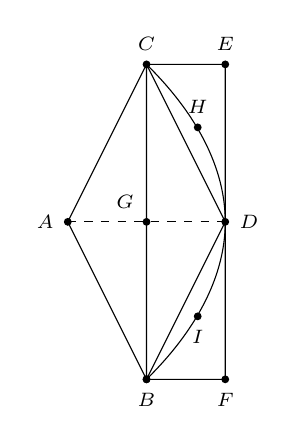
\begin{tikzpicture}
			\draw[] (0,0)node[circle,fill,inner sep = 1,label = below:\scriptsize$B$]{}--(1,0)node[circle,fill,inner sep=1pt,label = below:\scriptsize$F$]{}--(1,2)node[circle,fill,inner sep=1pt,label = right:\scriptsize$D$]{}--(1,4)node[circle,fill,inner sep=1pt,label = above:\scriptsize$E$]{}--(0,4)node[circle,fill,inner sep=1pt,label = above:\scriptsize$C$]{}--(-1,2)node[circle,fill,inner sep=1pt,label = left:\scriptsize$A$]{}--(0,0)node[circle,fill,inner sep=1pt]{}--(0,2)node[circle,fill,inner sep=1pt,label = above left:\scriptsize$G$]{}--(0,4)--(1,2)--(0,0);
			\draw[dashed](-1,2)--(1,2);
			\draw[rotate=90] (0,0) parabola bend (2,-1) (4,0);
			\draw[] (.65,.8)node[circle,fill,inner sep = 1,label = below:\scriptsize$I$]{};
			\draw[] (.65,3.2)node[circle,fill,inner sep = 1,label = above:\scriptsize$H$]{};
		    \end{tikzpicture}
		\end{center}
		\vspace{.5cm}

	    %---------- (c)
	    \item Demuestre que existe un polígono regular $P$ inscrito en un círculo y con área tan próxima como se desee al área del círculo.\\\\
		Demostración.-\;

	    %---------- (d)
	    \item Utilizando el hecho de que las áreas de dos polígonos regulares con el mismo número de lados están entre sí en la misma relación que los cuadrados de sus lados, demuestre que las áreas de dos círculos están en la misma relación que los cuadrados de sus radios.\\\\
		Demostración.-\;

	\end{enumerate}

\end{enumerate}

